% This file was created with tikzplotlib v0.10.1.post12.
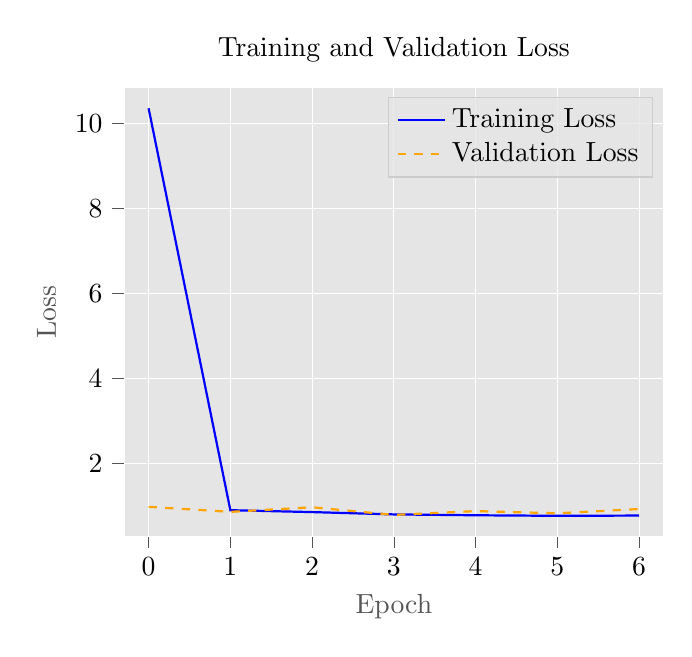
\begin{tikzpicture}

\definecolor{dimgray85}{RGB}{85,85,85}
\definecolor{gainsboro229}{RGB}{229,229,229}
\definecolor{lightgray204}{RGB}{204,204,204}
\definecolor{orange}{RGB}{255,165,0}

\begin{axis}[
axis background/.style={fill=gainsboro229},
axis line style={white},
legend cell align={left},
legend style={fill opacity=0.8, draw opacity=1, text opacity=1, draw=lightgray204, fill=gainsboro229},
tick align=outside,
tick pos=left,
title={Training and Validation Loss},
x grid style={white},
xlabel=\textcolor{dimgray85}{Epoch},
xmajorgrids,
xmin=-0.3, xmax=6.3,
xtick style={color=dimgray85},
y grid style={white},
ylabel=\textcolor{dimgray85}{Loss},
ymajorgrids,
ymin=0.28724604845047, ymax=10.8370169997215,
ytick style={color=dimgray85}
]
\addplot [thick, blue]
table {%
0 10.3574819564819
1 0.899181962013245
2 0.854719042778015
3 0.799882531166077
4 0.77983295917511
5 0.766781091690063
6 0.772865831851959
};
\addlegendentry{Training Loss}
\addplot [thick, orange, dashed]
table {%
0 0.97846120595932
1 0.860280930995941
2 0.968036293983459
3 0.787933230400085
4 0.877970337867737
5 0.826096415519714
6 0.926839411258698
};
\addlegendentry{Validation Loss}
\end{axis}

\end{tikzpicture}
